\documentclass[a4paper]{article}
\title{COMP1216 Coursework 1}
\author{Group 22\\ jrm2g19 (James Muir), cn4g18 (Chike Nwaenie), iko1g18 (Imisi Olubummo), wc1g19 (Bill Cao)}

\usepackage{geometry}
\geometry{
	a4paper,
	total={170mm,257mm},
	left=20mm,
	top=20mm,
}
 
\usepackage{graphicx}
\graphicspath{ {./images/} }
 
\begin{document}
	\maketitle
	\begin{center}
	\begin{itemize}
		\item jrm2g19 Parts 1, 2 and 3
		\item cn4g18 Parts 2 and 4
		\item wc1g19 Parts 3, 7 and 8
		\item iko1g19 Parts 5 and 6
	\end{itemize}
	\end{center}
	\newpage
	\section{Scope of the System}
	\subsection{Need}
	\begin{itemize}
		\item Improve interaction in lectures
		\item Provides feedback to lecturers about areas of poor understanding
	\end{itemize}	
	\subsection{Goals}
	\begin{itemize}
		\item To allow the host to run quizzes and users to answer them
		\item Obtain live feedback from students to quickly address areas of misunderstanding
		\item Engage students
	\end{itemize}
	\subsection{Business Case}
	\begin{itemize}
		\item The need of this new interactive quiz system is that it will provide lecturers
with invaluable feedback about whether students are understanding the content. It will also 
use gamification which will increase engagement from users.
	\end{itemize}
	\subsection{Stakeholders}
	\begin{itemize}
		\item Creator (lecturers/students)
		\item Users (students)
		\item Host
		\item Server administrators
		\item The University
	\end{itemize}	
	\subsection{High Level Operational Concepts}
	\begin{itemize}
		\item Server administrators will set up server package
		\item Creator will create quizzes of varying length and be able to edit the
		\item Host will set quizzes to run
		\item Users will answer questions on a running quiz
		\item Allow students to register
		\item A timer will provide a time-out on questions when:
		\begin{itemize}
			\item All participating players have answered the question
			\item The time for the question is up
			\item The host terminates the question early
		\end{itemize}
		\item Generate a unique number/code for users to connect
		\item Quiz provides a summary at the end of each question
		\item Quiz generates a report at the end of the quiz
	\end{itemize}	
	
	\newpage
	\section{Scenario}
	\subsection{Scenario One}
	A user signs in and creates a new quiz containing several multiple choice questions. After finishing the quiz, the user shares it with another registered user and logs out.	
	\begin{enumerate}
		\item The registered user(creator) signs in onto the welcome page
		\item The user selects the option to create a new quiz
		\item The user adds a new question
		\item The user selects the number of options and fills in the question and answer options
		\item The user selects the correct answer option
		\item The user sets the predefined timeout
		\item The user repeats step 3 to 6 until the user is happy and saves the quiz
		\item The user selects the option to share the quiz
		\item The user selects the user they want to share with and confirms
		\item The user logs out
	\end{enumerate}
	\subsection{Scenario Two}
	A host signs in a starts an existing quiz. The players join in and answer the questions.
	\begin{enumerate}
		\item The host signs in on the welcome page
		\item The host selects a defined quiz and a unique number is generated for it
		\item The users enter the generated number to join the quiz
		\item The host initiates the quiz
		\item The quiz goes through the predefined questions
		\item Each questions ends when the timer has run out, all users have answered or the host terminates the question prematurely
		\item A summary of answers to the question is displayed after each question ends
		\item Once all questions have been answered a summary is produced, displayed and saved to the host's account
	\end{enumerate}
	
	\newpage
	\section{Use Case Descriptions}
	\subsection{Use Case Description One}
	\subsubsection{Scope}
	A user signs in and creates a new quiz containing several multiple choice
questions. After finishing the quiz, the user shares it with another registered
user and logs out
	\subsubsection{Need}
	\begin{itemize}
		\item To test other user's understandings
		\item Provide engagement
	\end{itemize}
	\subsubsection{Primary Actor}
	\begin{itemize}
		\item User: who creates the quiz, shares it with another registered user and logs out
	\end{itemize}
	\subsubsection{Stakeholders}
	\begin{itemize}
		\item The University: The university will want to know whether Academic Integrity is being adhered to here,
having an unregulated quiz site could be a safe haven for illegitimately obtained or shared
answers. It could also have foul or obscene language which needs to be regulated.
		\item  The creator: The creator will want to know whether the quiz they made can be used by other students,
they will also want to know whether only the students they have shared quizzes with can
access the quizzes
		\item Registered users: They will want to be able to access quizzes shared with them
	\end{itemize}
	\subsubsection{Preconditions}
	\begin{itemize}
		\item The creator must be signed in
		\item The users that the creator intends to share the quiz with must be existing accounts
		\item All users must have internet connection
	\end{itemize}
	\subsubsection{Main Success Scenario}
	\begin{enumerate}
		\item The Creator logs in
		\item The Creator creates a New Quiz
		\item The Creator creates a New Question
		\item The Creator attaches one or more Answers to the Question
		\item The Creator repeats step 3 and 4 as many times as desired
		\item The Creator can either Save or Exit without Saving
		\item The Creator specifies which user(s) they wish to share the quiz with
		\item The Creator may sign out
		\item A Registered User signs in
		\item A Registered User can access the Quiz
	\end{enumerate}
	\subsubsection{Extensions}
	\begin{enumerate}
		\item What could go wrong?
		\begin{itemize}
			\item The Creator may not remember their username/password, and thus will not be allowed to sign in
			\item The Quiz may be of corrupt format meaning the Creator cannot save/the user cannot access the quiz
			\item The Quiz may not be saved properly due to incorrect choice, power cut, database crash, etc.
		\end{itemize}
	\end{enumerate}
	
	 \subsection{Use Case Description Two}
	\subsubsection{Scope}
	A system which allows a host to start an existing quiz, which also
	allows the players join in and answer questions.
	\subsubsection{Need}
	\begin{itemize}
		\item This is needed so that control is alloted for the user to begin the quiz and so
		players can join the quiz and answer questions
	\end{itemize}
	\subsubsection{Primary Actor}
	\begin{itemize}
		\item Host: who starts the quiz
	\end{itemize}
	\subsubsection{Stakeholders}
	\begin{itemize}
		\item  Host: The host want to confirm that the quiz has begun
		\item  The players: The players will want to be able to join in and answer
		\item  The University: They will want to monitor what questions are being asked for ethical and academic
		integrity.
	\end{itemize}
	\subsubsection{Preconditions}
	\begin{itemize}
		\item The host must be signed in
		\item The players must be signed in
	\end{itemize}
	\subsubsection{Main Success Scenario}
	\begin{enumerate}
		\item The Host logs in
		\item The Host starts an existing Quiz giving time for players to join
		\item A new question is issued
		\item Players are allowed to answer
		\item Step 3 and 4 are repeating as many times as necessary
		\item The Host may sign out
		\item The players may signs out
	\end{enumerate}
	\subsubsection{Extensions}
	\begin{enumerate}
		\item What could go wrong?
		\begin{itemize}
			\item The Host may not remember their username/password, and thus will not be allowed to sign in
			\item The code/key supplied so that players can join the game may be improperly typed/faulty, not allowing
			players to join the game
			\item The answer options may be unresponsive
		\end{itemize}
	\end{enumerate}
	
	\newpage
	\section{Use Case Diagram}
	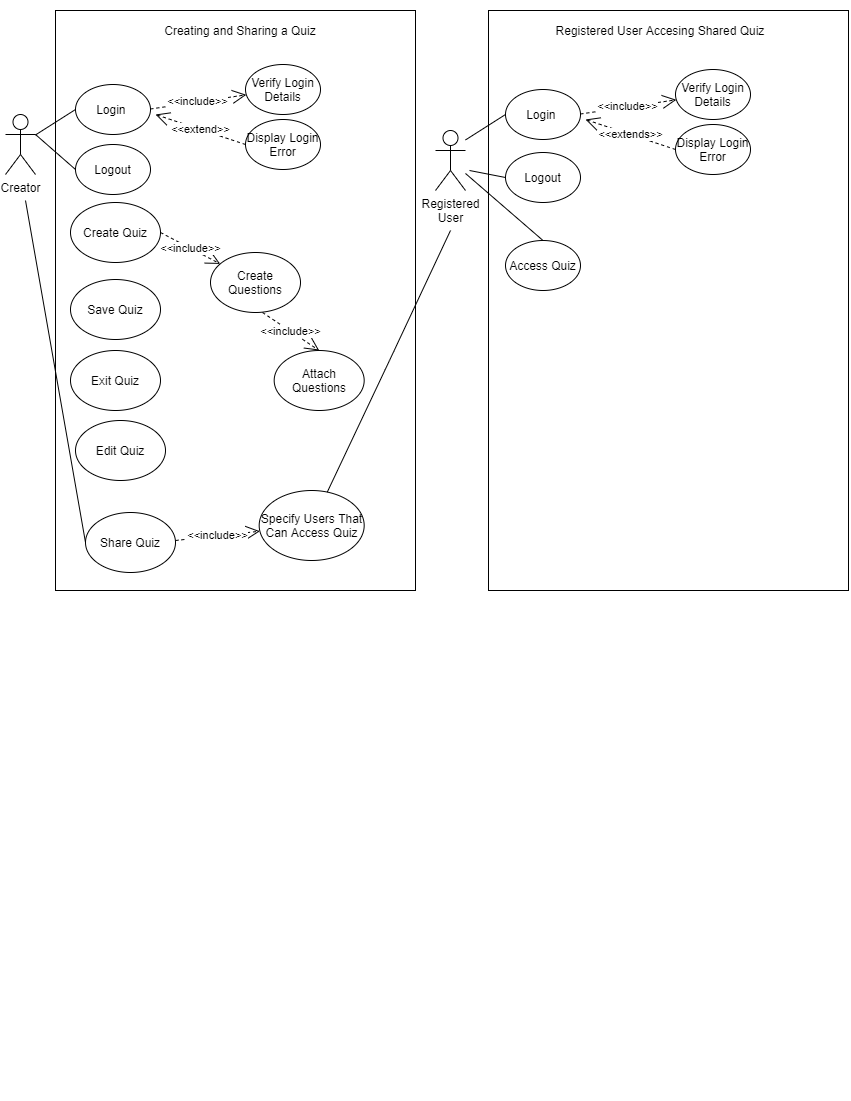
\includegraphics[scale=0.55]{Login_Create_Quiz_Use_Case_Diagram}

	\newpage
	\section{Class Diagram}
	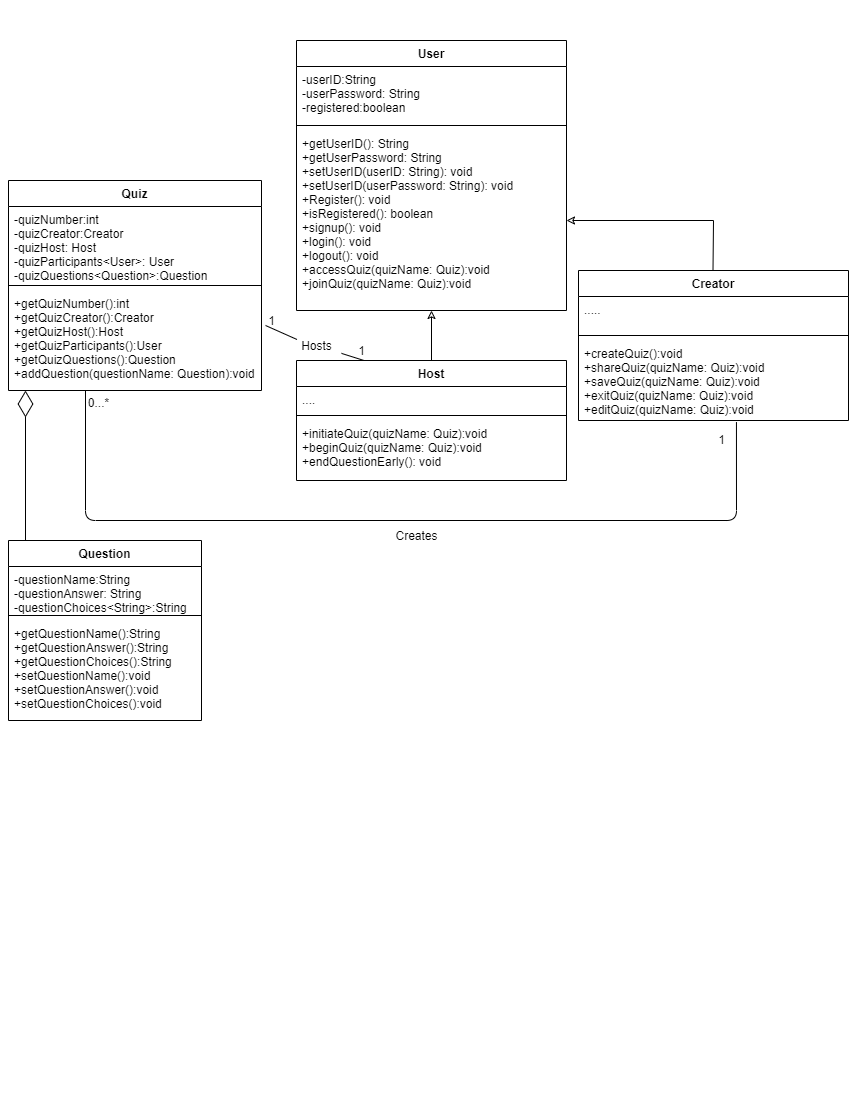
\includegraphics[scale=0.55]{Class_Diagram}
	
	\section{Sequence Diagrams}
	\subsection{Sequence Diagram 1}
	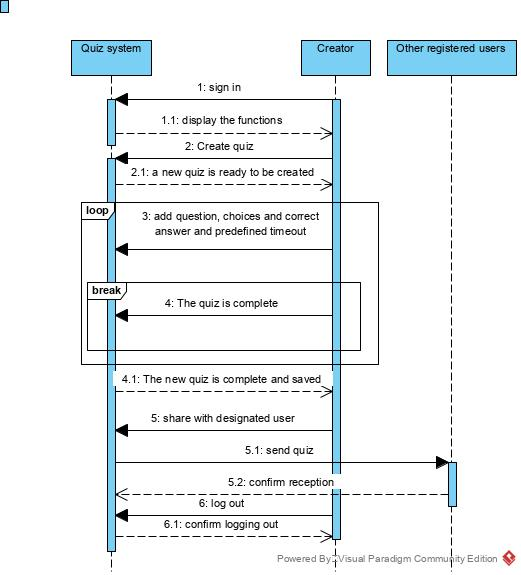
\includegraphics[scale=1]{Sequence_Diagram1}
	\subsection{Sequence Diagram 2}
	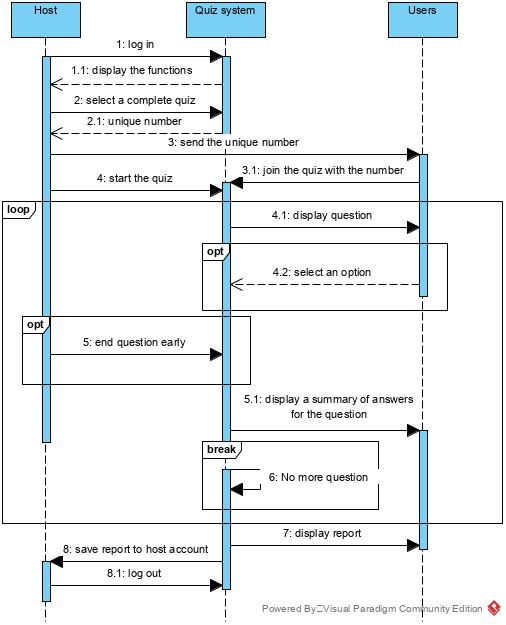
\includegraphics[scale=1]{Sequence_Diagram2}
	
	\newpage
	\section{Activity Diagram}
	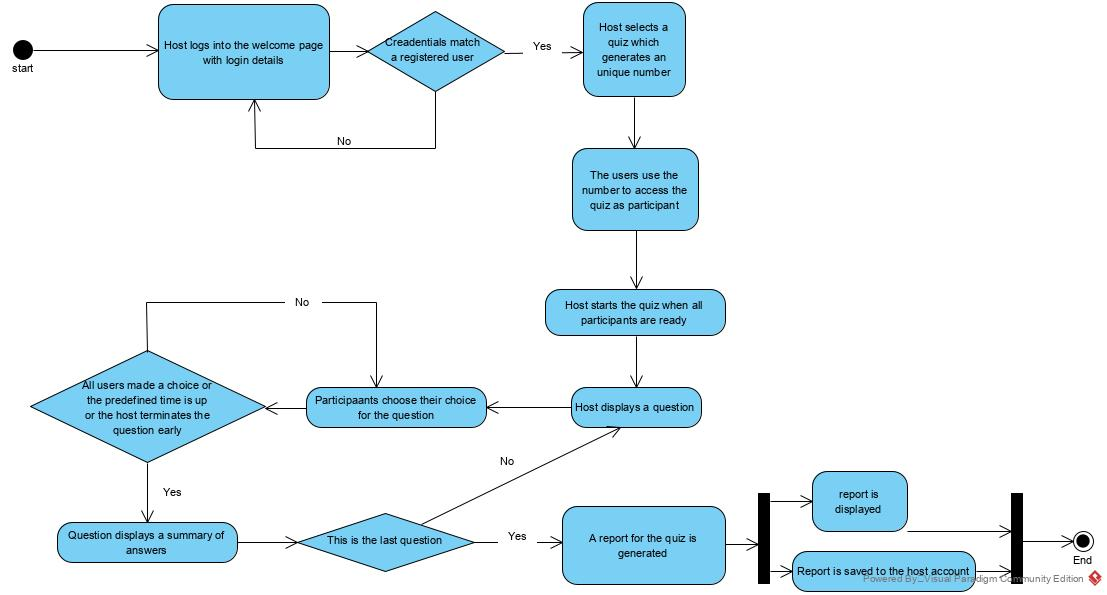
\includegraphics[scale=0.6]{Activity_Diagram1}
\end{document}